% A chapter: heading, sections, a citation, a figure, a table, an equation, and
% its own reference list. Copy this file for each chapter.
\chapter{Elements of a Chapter}
\label{ch:example}

\section{Abstract}
\label{sec:example:abstract}

In a manuscript style dissertation, a chapter that reproduces a paper opens with the paper's abstract. Otherwise delete this section.

\section{Text and citations}
\label{sec:example:text}

The template sets the body at 1.5 line spacing in a sans serif font with no first line indent, as the 2027 University Dissertation and Thesis Services (UDTS) rules require. Paragraphs are separated by a blank line in the source.

Citations use the apacite package in the author and year form. A citation inside a sentence looks like this \cite{bor_systematic_2026}. When the authors are the subject of the sentence, \citeA{oughton_major_2026} reported the result. The reference list of each chapter contains only the works cited in that chapter. Section~\ref{sec:example:figure} shows a figure, Section~\ref{sec:example:table} a table, and Section~\ref{sec:example:equation} two equations.

An abbreviation is written out at its first use in each chapter, for example geomagnetically induced currents (GICs), and abbreviated afterwards. The front matter lists every abbreviation and symbol.

\section{A figure}
\label{sec:example:figure}

Every figure needs alternative text for screen readers. It goes in the \verb|alt| key of the graphics command, as in the source of this file. Figure files can be PDF or PNG. The short caption in square brackets goes to the List of Figures. Figure~\ref{fig:example:mason} shows the layout.

\begin{figure}[htbp]
  \centering
  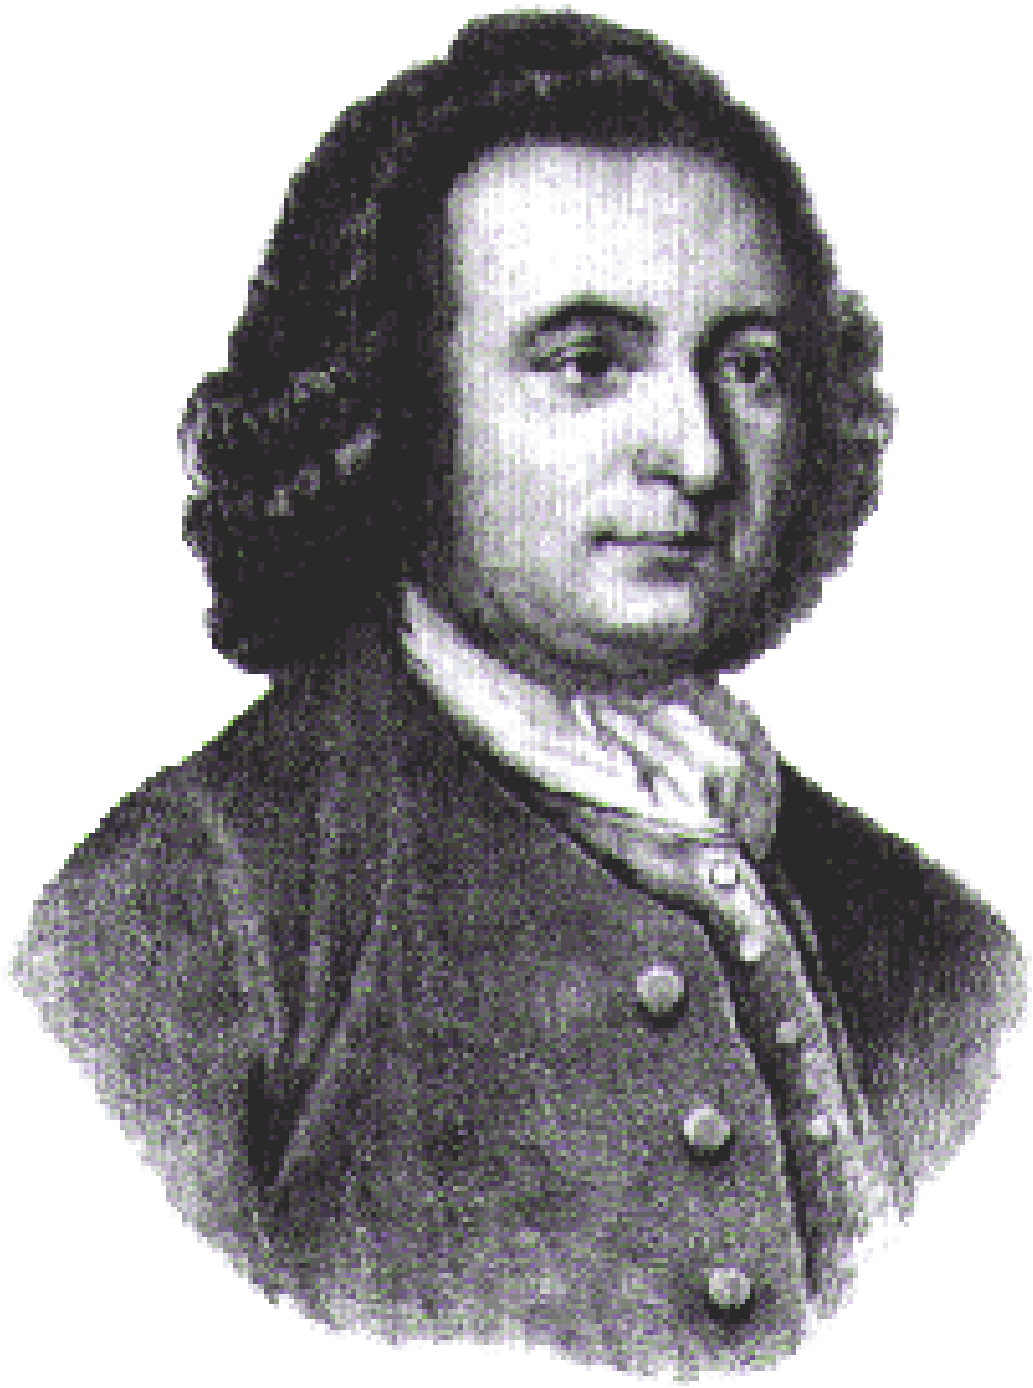
\includegraphics[width=0.5\linewidth,keepaspectratio,
    alt={The George Mason University seal.}]
    {figures/figGeorgeMason.pdf}
  \caption[The George Mason University seal]
  {The George Mason University seal, the example figure supplied with the UDTS template. Describe what the figure shows and name the source of the image.}
  \label{fig:example:mason}
\end{figure}

\section{A table}
\label{sec:example:table}

The caption of a table sits above it. The \verb|\tagpdfsetup| line marks the header row so the PDF records the table structure. Table~\ref{tab:example:values} gives example values.

\begin{table}[htbp]
  \centering
  \caption[Example values by case]
  {Example values by case. Units are in the column headings.}
  \label{tab:example:values}
  \tagpdfsetup{table/header-rows={1}}
  \begin{tabular}{lrr}
    \hline
    Case & Voltage (V) & Current (A) \\
    \hline
    A & 120 & 2.0 \\
    B & 240 & 1.5 \\
    C & 480 & 0.8 \\
    \hline
  \end{tabular}
\end{table}

\section{Equations}
\label{sec:example:equation}

Equations are numbered by chapter. The sentence after an equation defines every symbol in it. Ohm's law relates voltage, current, and resistance,
\begin{equation}
  V = I R,
  \label{eq:example:ohm}
\end{equation}
where $V$ is the voltage in volts, $I$ the current in amperes, and $R$ the resistance in ohms. The sample mean of $n$ observations is
\begin{equation}
  \bar{x} = \frac{1}{n} \sum_{i=1}^{n} x_i,
  \label{eq:example:mean}
\end{equation}
where $x_i$ is the $i$th observation. Both equations appear in the List of Equations through their labels.

\chapterreferences
